\chapter{Results \& discussion}
\label{ch:Results discussion}
\begin{figure}
  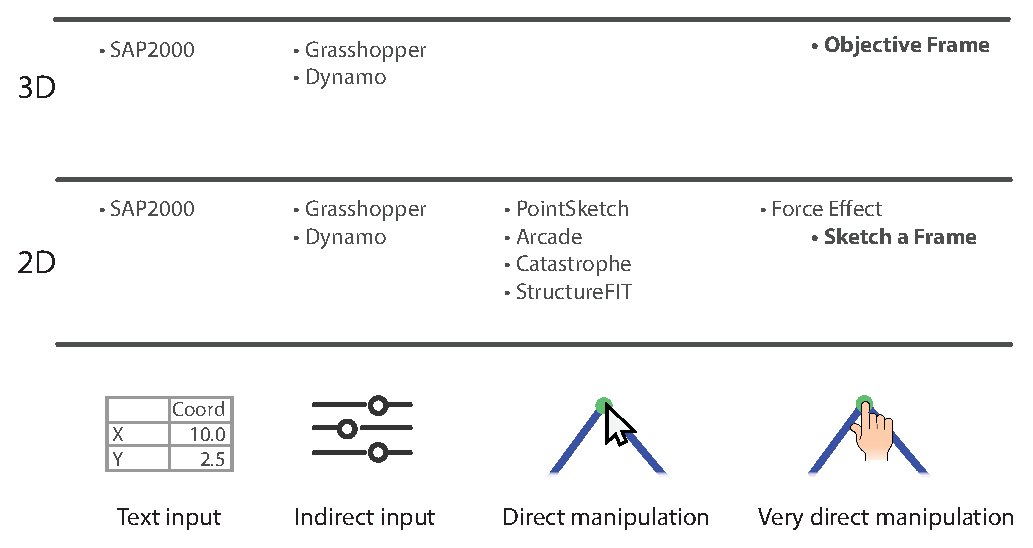
\includegraphics[width=330pt]{graphics/softwareReview.eps}
  \caption{Previous work summarized, present work in bold}
  \label{fig:softwareReview}
\end{figure}

A summary of the evaluated conceptual design tools can be seen in Figure \ref{fig:softwareReview}, where the tools are grouped according to the number of dimensions and the manipulation experience. The two developed applications have a higher degree of direct manipulation in 2D and 3D than other existing software for conceptual design. This has been achieved by using novel technology: the multi-touch user interface for 2D and the Leap Motion Controller for 3D.

This thesis responds to a need for new, more intuitive and natural interaction modes in computational design and analysis. Very direct manipulation represents a significant improvement on the direct manipulation paradigms that are prevalent in CAD. New technologies like the Leap Motion Controller and the multi-touch interface open up unprecedented possibilities for engaging users in the exploration and design of structures. This will improve users’ understanding of the structural behavior of a model and their cognitive engagement in the task performed, and encourage further design exploration.


\section{Summary of intellectual contributions}
\begin{itemize} 
\item This thesis includes a critical review of existing tools and techniques for design manipulation in conceptual CAD.
\item Paper A proposes a new direct manipulation cycle that automatically computes and presents the result once a structure is stable.
\item Paper A introduces new multi-touch interaction models for conceptual structural design on tablets.
\item Paper B describes the first method for very direct manipulation as a human--computer interaction mode for 3D structures, based on new 3D input devices such as the Leap Motion Controller.
\item Paper B introduces a design tool that allows users to interact with 3D structures through very direct manipulation.
\item Paper B demonstrates the potential applications of 3D input devices through three case studies.
\end{itemize} 


\section{Future work}
The Leap Motion Controller’s SDK supports virtual reality glasses such as the Oculus Rift. Combining the two could create a virtual reality application in which users can experience the structure in 3D, interact with it, and make changes using their hands. 

This could potentially be developed in a game environment, where the structure is visualized in the intended context, i.e., the building site. A game engine would enable real-time renderings of the structure within this context. Designers would then be able to perform manipulations, guided by performance feedback, on the rendered structure. 

Other existing design methods could be combined with this design environment, such as interactive optimization with the use of genetic algorithms. To improve the computation speed and allow the rapid generation of new designs, the design space could be approximated with the help of artificial neural networks, also known as surrogate modeling. This would allow for more advanced structural models to be used for interactive optimization.

Finally, it is necessary to evaluate and, if possible, also quantify the impact of the conceptual structural design tools on the design process. Therefore, it is important to perform case studies in future work.

